\chapter{Concept\label{cha:chapter3}}
\section{Communication between Object Detection System and Client}
If two humans want to communicate with one another, they need matching channels and they need to speak the same language. A channel is a mean of transport for information, e.g. sign language, smoke signs, mobile phones etc. If one entity tries to call someone via phone if the other does not have a phone, the caller enters the wrong number, the other has its phone turned off, they cannot communicate. In case they both have a phone, the called entity answers and both speak a common language (e.g. English), exchange of information can be achieved. Communication within technical systems faces the same challenges. As for the right channel, models like the OSI basic reference model for information technology standardized by ISO layer the transfer of information from the physical layer consisting of peaks in currents and voltages up until the application layer which includes direct user interaction, resource availability and so forth. \cite{InternationalOrganizationForStandardization1996ISO/IECEd.} This model and the protocols adhering to it ensure that information is delivered safely between communicating entities. However, this model does not imply the semantics of the payload or the language as stated in the analogy above. A currently proposed semantic standard for OD processes is \textbf{OPC UA Vision}. It includes a finite state machine abstracting an industrial system from its diverse conditions and transitions. Moreover it offers an information model covering the administration of recipes, configurations and results. With the help of the state machine it is defined which information of the information model is retrievable. The content of the three administration objects remain proprietary with the advantage of covering a broad range of OD scenarios.\\

According to the specification, powering up and shutting down a vision system are mandatory processes and thus should be handled in a standardized manner. Also, the handling of errors should be the same for all vision systems. The design of the core operation state however shall remain with the manufacturer. Automatic mode as sub-state of operational mode as   is one proposed way of designing it. It reflects the goal of specifying a system to be easily integrated into automated production and inspection systems. An example for this operation would be a PLC guiding an inspection system for position determination. The state machine for a typical vision system is depicted in \ref{fig:OPCStateMachineAutomatic}. When powered on, the system enters the preoperational state through loading a configuration marked as active. From there an operation mode is either automatically chosen by the system or manually triggered. An operation mode is any sub-state machine of the operational state. The automatic mode is chosen and enters the initial state. Then a recipe can be prepared, describing properties, procedures and parameters for a machine vision job. The recipe may include information for a single and / or continuous execution. A single execution would be e.g. determining the pose of an object, a continuous execution could be monitoring and surveillance systems which constantly process and acquire data. When the system is done with an execution or execution step, e.g. taking a picture from one of four angles, it sends results asynchronously to the client. If the system is shut down, it should be put into the halt mode first where a safe power off is assured. From all states it is possible to enter the error state. Errors are handled aligning with their severity and sometimes need acknowledgement or confirm by a human, before the system can be reset to preoperational state.\\

\begin{figure}[ht]
    \centering
    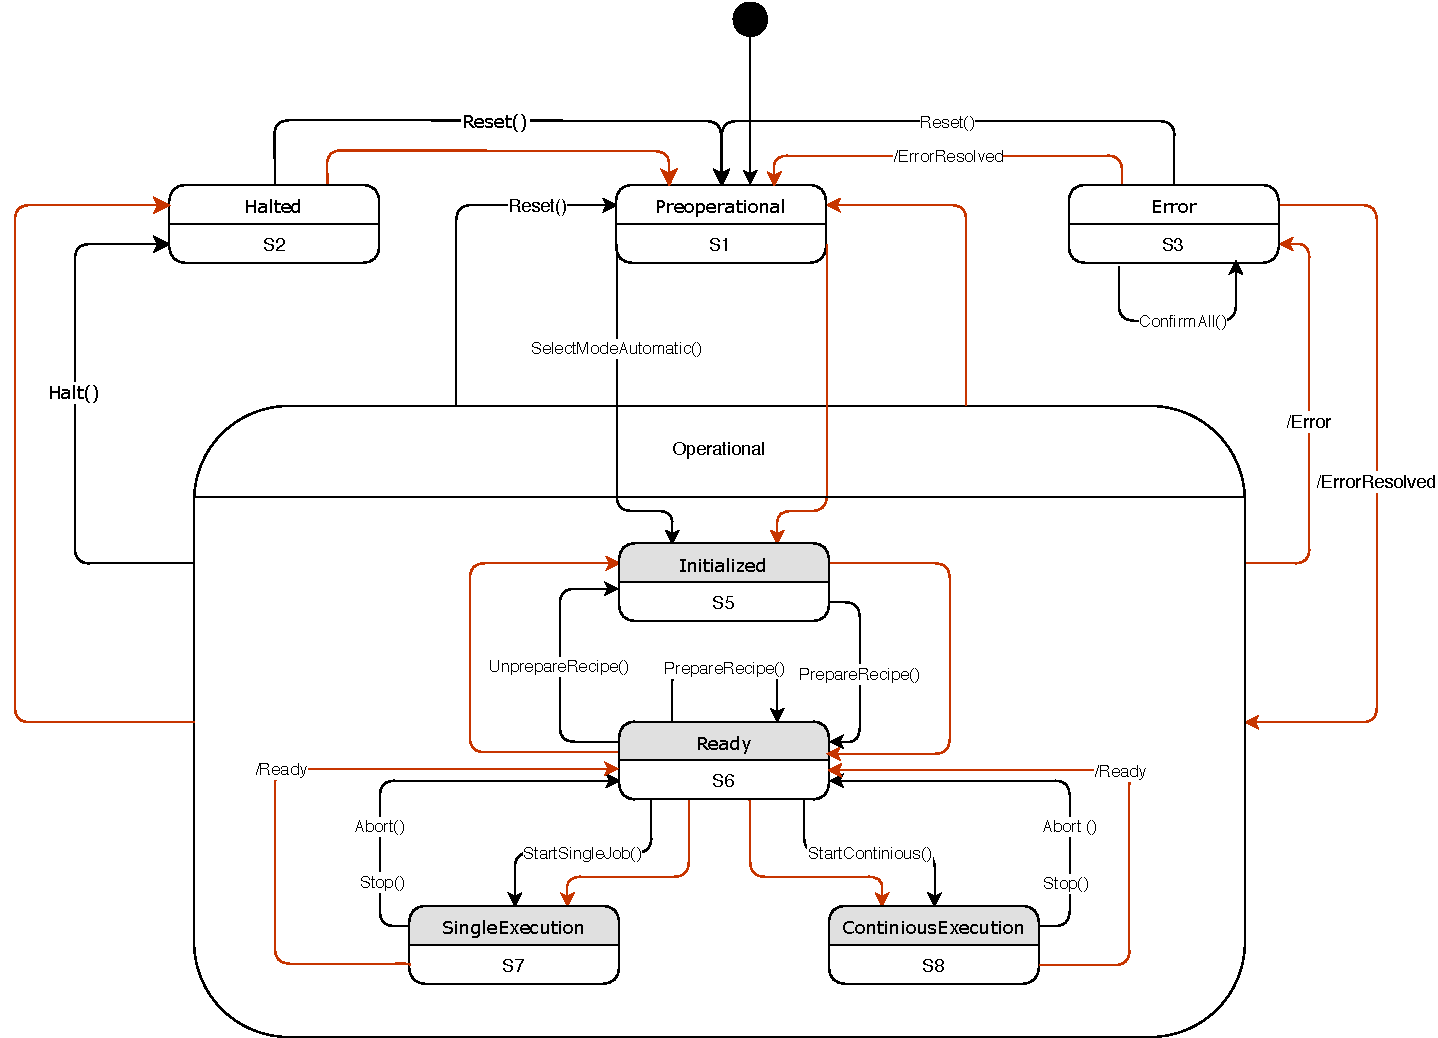
\includegraphics[width=\textwidth]{img/OPCUAVisionVisionAutomaticModeStateMachineStates.pdf}
    \caption[OPC UA Vision state machine in automatic operation mode]{OPC UA Vision state machine in automatic operation mode. Red Lines indicate automatic transitions induced by the vision system with optional effects prefixed with a slash. Black lines indicate method induced transitions with the method name as trigger. The black circle is the entry point of the state machine. All of the states can have optional sub-state machines. States marked in grey are substates.\cite{VDMA2018OPCSpecification}}
    \label{fig:OPCStateMachineAutomatic}
\end{figure}

The information model formally describes all datasets, types, methods, address- and namespaces. See fig. \ref{fig:OPCInfoModelOverview} for an overview and \ref{fig:OPCInfoModelNotation} for an explanation of the notation. The StartSingleJob method (not depicted in the overview) for example triggers transisition from state Ready to SingleExecution in \ref{fig:OPCStateMachineAutomatic}. Its signature consists of following parameters:

\begin{tabbing}
    space \= space \= spacespacespace \= spacespacespacespace \= spacespacespace \kill
    \>  StartSingleJob(\\
    \>  \>  (in)	 \> 	String          \> MeasId\\
    \>  \>  (in)	 \> 	String          \> PartId\\
    \>  \>  (in)	 \> 	RecipeIdType    \> RecipeId\\
    \>  \>  (in)	 \> 	ProductIdType   \> ProductId\\
    \>  \>  (out)	 \> 	String          \> JobId\\
    \>  \>  (out)	 \> 	Int32           \> Error); 
\end{tabbing}

\begin{figure}
    \centering
    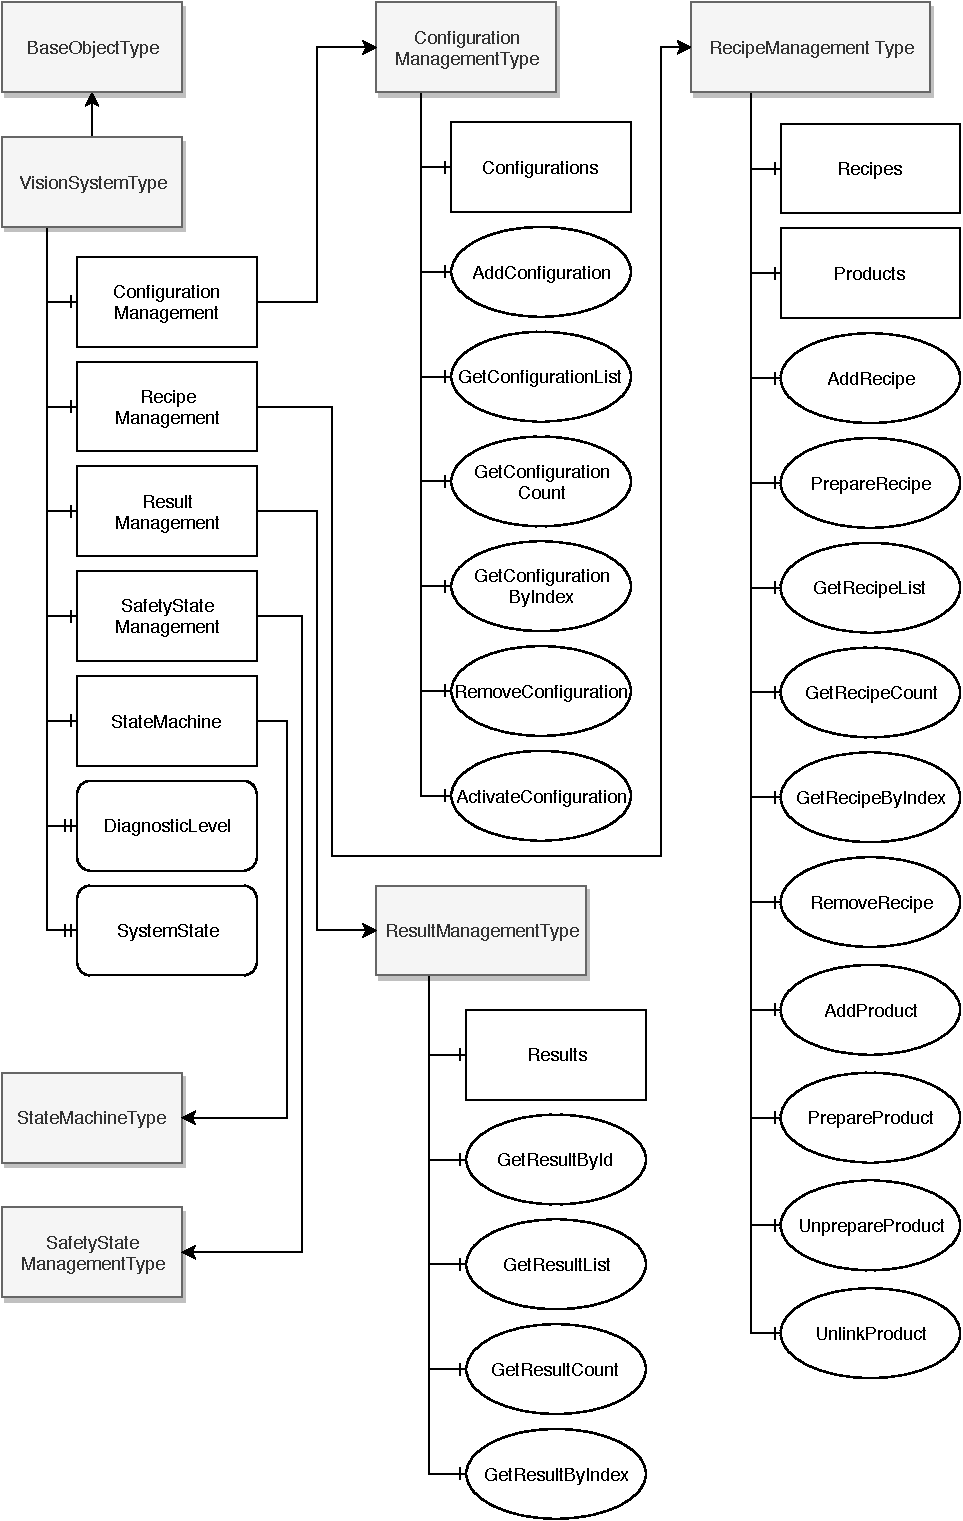
\includegraphics[height=0.9\textheight]{img/OPCUAVisionInformationModelOverview.pdf}
    \caption[OPC UA Vision Information Model Overview]{OPC UA Vision Information Model Overview. See fig. \ref{fig:OPCInfoModelNotation} for a description of the notation.\cite{VDMA2018OPCSpecification}}
    \label{fig:OPCInfoModelOverview}
\end{figure}

\begin{figure}[ht]
    \centering
    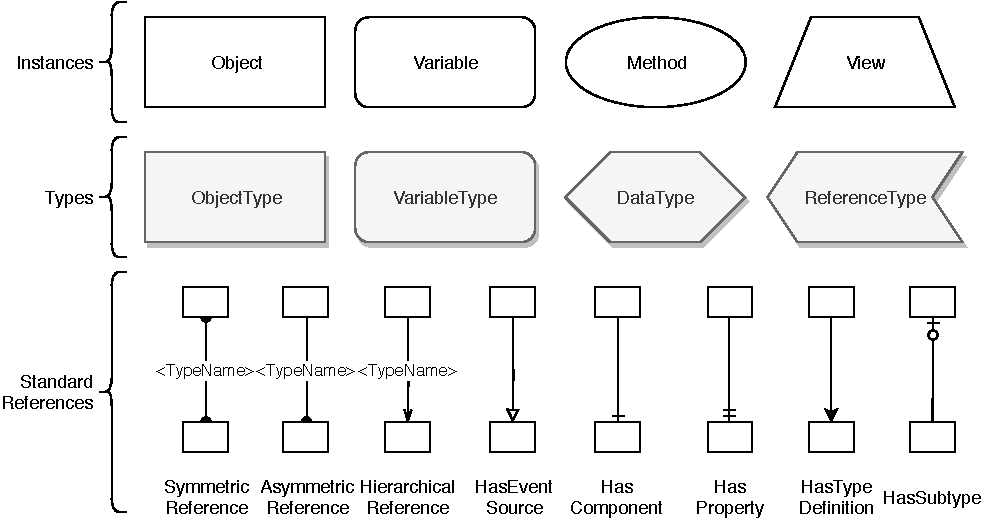
\includegraphics[width=0.8\textwidth]{img/OPCUAVisionInformationModelNotation.pdf}
    \caption[OPC UA Vision Information Model Notation]{OPC UA Vision Information Model Notation.\cite{VDMA2018OPCSpecification}}
    \label{fig:OPCInfoModelNotation}
\end{figure}

The generated OD services should adhere to the OPC UA Vision companion specification. 
\section{Service Generation}
\subsection{Object Detection Method Integration}

\begin{figure}[ht]
    \centering
    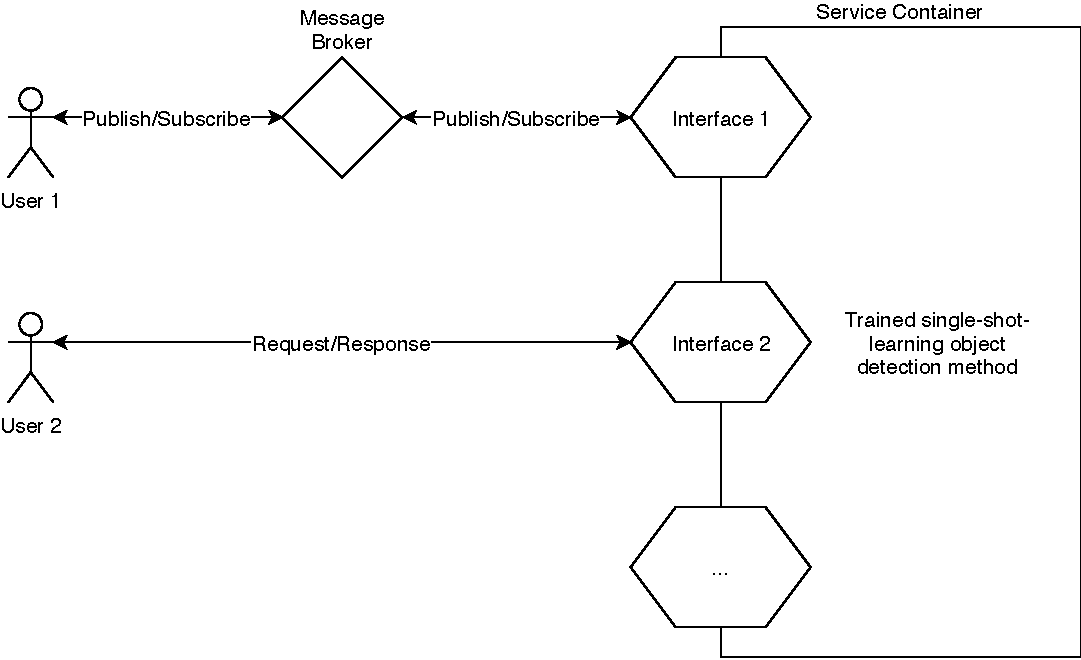
\includegraphics[width=0.8\textwidth]{img/ServiceArchitecture.pdf}
    \caption{Service Interface Architecture.}
    \label{fig:ServiceInterArchit}
\end{figure}

\begin{figure}[ht]
    \centering
    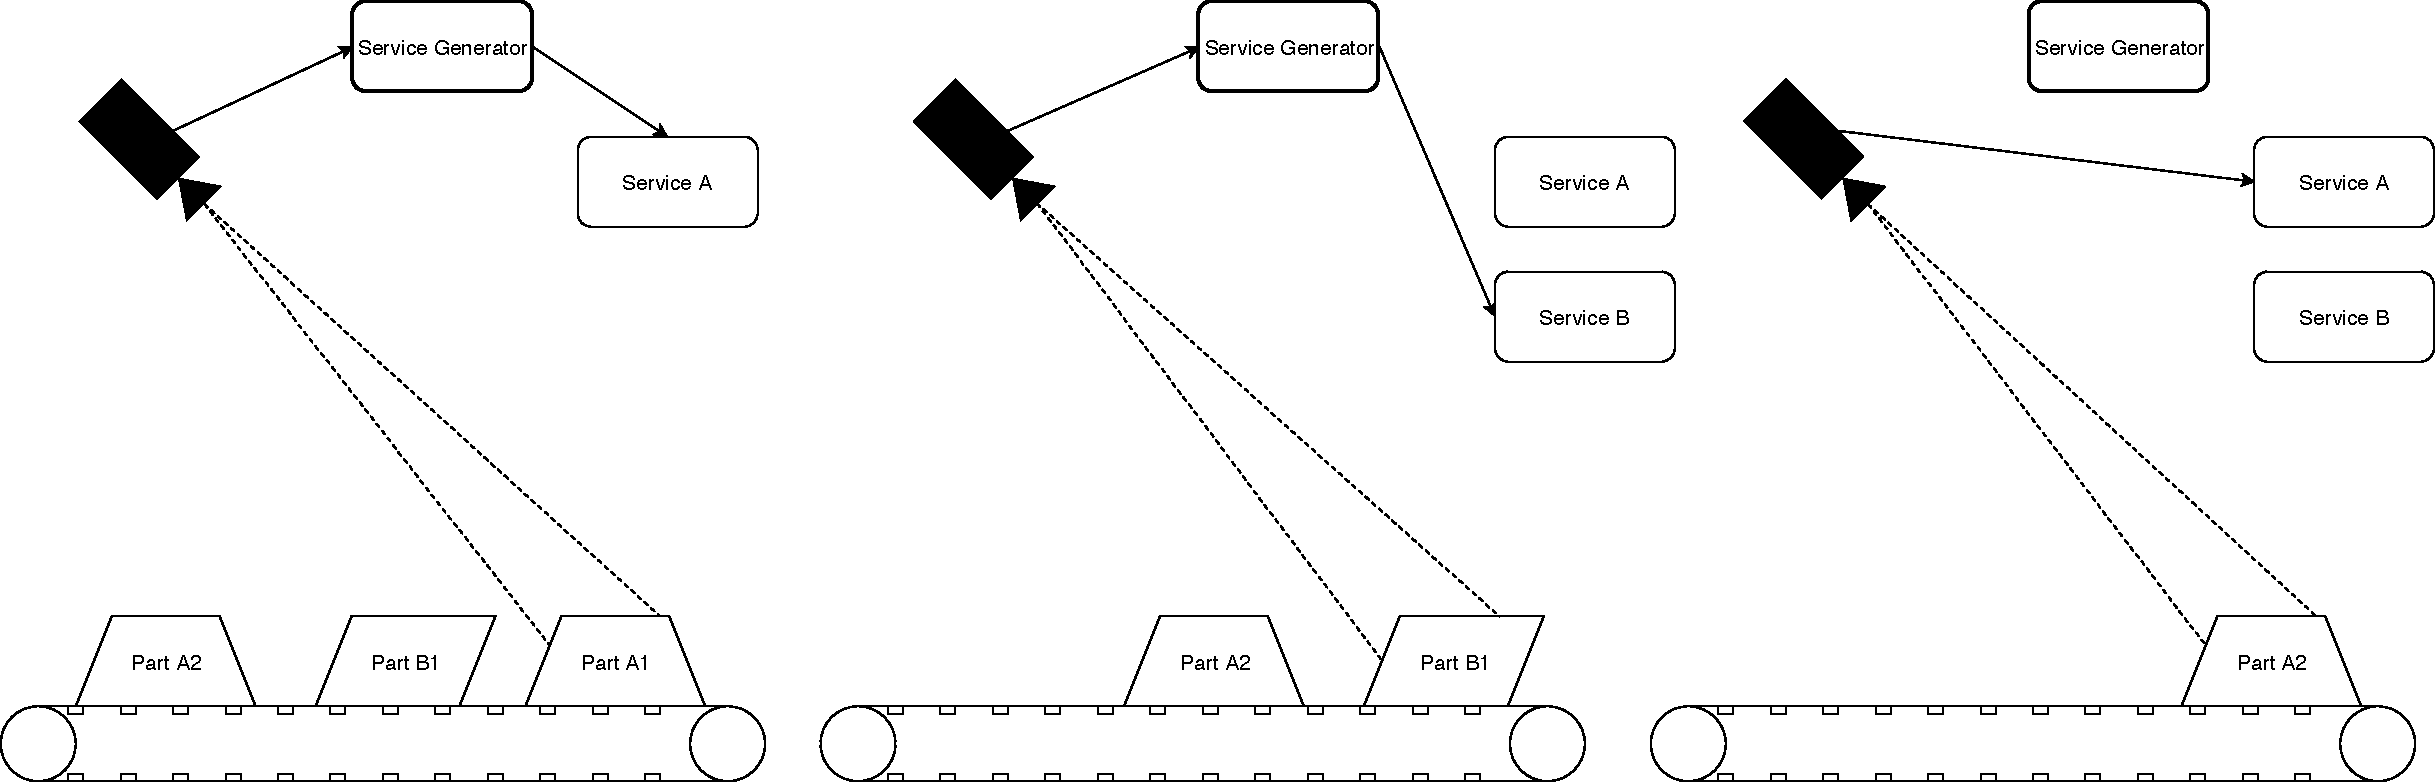
\includegraphics[width=0.8\textwidth]{img/ServiceGenerationExample.pdf}
    \caption{Service generation example in industrial context.}
    \label{fig:ServiceGenExa}
\end{figure}

\subsection{Interface Definition and Protocol Adapters}
For client usability reasons it is beneficial if a service is addressable via several protocols. For example a service using GRPC based on http/2 might want to interact with older web clients which use REST based on http/1.1. IoT devices sometimes only support lightweight publish-subscribe protocols such as MQTT. 
\section{Evaluation Parameters}
As opposed to monolithic applications SOAs are highly agile and easily integrated into distributed systems. This hypothesis has to be supported by qualitative and quantitative test results. An example for a qualitative test would be a test center where the same OD algorithm has to be integrated into a SOA and a monolithic application. The integration should be executed by several equally skilled groups of which one half start with the SOA and the other with the monolithic application. 
Quelle mit Evaluierfragen heranziehen.
Quantitative parameters could be the size of the service containers, the CPU and RAM load they utilize. The usability of the service is also of high impartance, e.g. the number of protocols that the interface offers, the documentation of the interface etc. 